% !TEX encoding = UTF-8 Unicode
% $Header: /cvsroot/latex-beamer/latex-beamer/solutions/conference-talks/conference-ornate-20min.en.tex,v 1.6 2004/10/07 20:53:08 tantau Exp $

\documentclass{beamer}

\mode<presentation>
{
  \usetheme{Warsaw}
  % or ...

  \setbeamercovered{transparent}
  % or whatever (possibly just delete it)
  
  \setbeamertemplate{navigation symbols}{}
  
  \newcommand*\oldmacro{}%
  \let\oldmacro\insertshorttitle%
  \renewcommand*\insertshorttitle{%
    \oldmacro\hfill%
    \insertframenumber\,/\,\inserttotalframenumber}
}

\usepackage[utf8]{inputenc}
% or whatever

\usepackage{times}
\usepackage{multirow}
\usepackage[T1]{fontenc}
\usepackage[french]{babel}
\usepackage{graphicx}
\usepackage{eso-pic}
\usepackage{color}
\usepackage{tikz}
\usepackage{wasysym}

% Or whatever. Note that the encoding and the font should match. If T1
% does not look nice, try deleting the line with the fontenc.

\title[Noosphère]
{}

\titlegraphic{\raisebox{2em}{}}

\author[Prologin]
{\includegraphics{../prologin2015}}

\date
{}

\begin{document}

\definecolor{vert}{rgb}{0.07 0.54 0.07}


\begin{frame}
%	\frametitle{PUROGURAMU}
	\vspace{0.5cm} \centering \includegraphics[width=0.9\linewidth]{../prologin2015}
\end{frame}

\begin{frame}
	\frametitle{Présentation}
	\begin{itemize}
        \item Jeu de stratégie à 2 joueurs : \textcolor{green}{Vert} et
            \textcolor{blue}{Bleu}
        \item Tour par tour
        \item Carte carrée de taille fixe
	\end{itemize}
\end{frame}

\begin{frame}
	\frametitle{Agent}
	\begin{itemize}
        \item Unité unique
        \item Déplaçable sur toute la carte
        \item Déclenche les actions du jeu
	\end{itemize}
\end{frame}

\begin{frame}
	\frametitle{Portails}
    \begin{columns}[T]
        \begin{column}{.3\textwidth}
            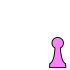
\includegraphics[width=3cm]{portal}
        \end{column}
        \begin{column}{.7\textwidth}
            \begin{itemize}
                \item Répartis sur la carte
                \item \textcolor{gray}{Neutres}, \textcolor{green}{Verts} ou \textcolor{blue}{Bleus}
                \item Peuvent être capturés
                \item Peuvent être neutralisés
                \item Peuvent être protégés avec des boucliers
            \end{itemize}
        \end{column}
    \end{columns}
\end{frame}

\begin{frame}
    \begin{center}
        \frametitle{Les portails}
        \includegraphics[height=0.8\textheight]{gui_empty}
    \end{center}
\end{frame}

\begin{frame}
	\frametitle{Lien}
    Il est possible de relier (\textbf{lien}) deux portails si :
	\begin{itemize}
        \item Votre agent se trouve sur un des deux portails
        \item Les deux portails vous appartiennent
        \item Aucun lien n'intersecte le lien à créer
        \item Aucun lien ne se superpose au lien à créer
        \item Aucun des deux portails n'est à l'intérieur d'un champ
	\end{itemize}
\end{frame}

\begin{frame}
    \begin{center}
        \frametitle{Le Jeu}
        \includegraphics[height=0.8\textheight]{gui_link}
    \end{center}
\end{frame}

\begin{frame}
	\frametitle{Cas particuliers}
    \begin{center}
    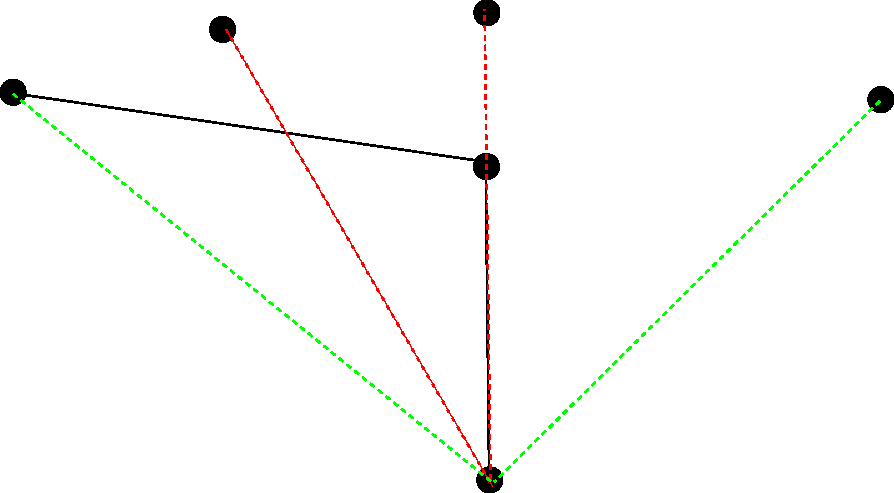
\includegraphics[height=0.7\textheight]{interference.pdf}
    \end{center}
\end{frame}


\begin{frame}
	\frametitle{Champ de contrôle}
    \begin{itemize}
        \item Trois portails reliés entre eux forment un \textbf{Champ de contrôle}
        \item Tous les triangles sont comptées
        \item Score gagné selon leurs aires
    \end{itemize}
\end{frame}

\begin{frame}
    \begin{center}
        \frametitle{Champs de contrôle}
        \includegraphics[height=0.8\textheight]{gui_triangle}
    \end{center}
\end{frame}

\begin{frame}
    \begin{center}
        \frametitle{Regardez c'est incroyable}
        \includegraphics[height=0.8\textheight]{gui_full}
    \end{center}
\end{frame}

\begin{frame}
	\frametitle{Score}
	\begin{itemize}
	\item[+] capturer un portail
    \item[+] aire totale contrôlée à la fin de chaque tour
	\end{itemize}
\end{frame}

\begin{frame}
	\frametitle{Points d'actions}
	\begin{itemize}
	\item[+] commencer un tour
	\item[\alert{--}] neutraliser un portail
	\item[\alert{--}] capturer un portail
	\item[\alert{--}] créer un lien
	\item[\alert{--}] utiliser un turbo
	\item[\alert{--}] poser un bouclier
	\end{itemize}
\end{frame}

\begin{frame}
	\frametitle{Points de déplacement}
	\begin{itemize}
	\item[+] commencer un tour
	\item[+] utiliser un turbo
    \item[\alert{--}] se déplacer (distance de Manhattan)
	\end{itemize}
\end{frame}

\begin{frame}
	\frametitle{Cas particuliers}
    \begin{center}
    
\includegraphics[height=0.7\textheight]{../triangle3.pdf}
    \end{center}
\end{frame}

%\begin{frame}
%	\frametitle{Cas particuliers}
%    \begin{center}
%    \includegraphics[height=0.7\textheight]{sierpinski1}
%    \end{center}
%\end{frame}
%\begin{frame}
%	\frametitle{Cas particuliers}
%    \begin{center}
%    \includegraphics[height=0.7\textheight]{sierpinski2}
%    \end{center}
%\end{frame}
%\begin{frame}
%	\frametitle{Cas particuliers}
%    \begin{center}
%    \includegraphics[height=0.7\textheight]{sierpinski3}
%    \end{center}
%\end{frame}
\begin{frame}
    \frametitle{Conférences}
    \begin{itemize}
        \item Vendredi 16h00 -- 16h30 : \emph{Programmation dynamique}
            -- Jill-Jênn Vie
        \item Vendredi 16h30 -- 17h00 : \emph{Programmation linéaire} --
            Nicolas Bonifas
        \item Vendredi 22h00 -- 22h30 : \emph{Droits des associations} -- Marin
            Hannache
        \item Samedi 14h00 -- 14h45 : \emph{Les déterminants en géométrie
            algorithmique} -- Sarah Fachada
        \item Samedi 14h45 -- 15h30 : \emph{Graphes planaires} -- Nicolas
            Blanchard
    \end{itemize}
\end{frame}
\end{document}
